\section{Forudsigelse af indlæggelsesvarigheden}
Ved ortopædkirurgiske operationer er der flere parametre, der kan have indflydelse på
indlæggelsesvarigheden. Dette kan eksempelvis være demografiske parametre såsom
alder samt køn og kliniske parametre som blodprøver, blodtab og operationstype. Da
der kan opstå komplikationer under en operationen, som kan have indflydelse på
indlæggelsesvarigheden opdeles parametrene præ- og postoperativt.


\subsection{Præoperativt}
På ortopædkirurgisk afdeling estimeres indlæggelsesvarigheden ikke på nuværende tidspunkt, dog vurderes indlæggelsesforløbet ud fra personalets erfaringer. Ud fra informationspjecer fra ortopædkirurgisk afdeling på Aalborg Universitetshospital informeres om, hvilke faktorer der kan være under en operation. Disse kan angiveligt forlænge indlæggelsesvarigheden. 


\subsubsection{Livsstilsfaktorer}
Livsstilsfaktorer tyder på at have betydning for komplikationer under en operation. Lavt præoperativt funktionsniveau og muskeltab er ofte aldersbetinget, hvilket kan medføre komplikationer og lang indlæggelsesvarighed. Hvorimod patienter med højt funktionsniveau ofte har kortere indlæggelsesvarighed.\cite{Kehlet2001, Janssen2002} Af \figref{alderogindlaeggelse} fremgår patientens alder samt indlæggelsesvarighed i perioden 1. august til den 31. oktober år 2014.


\begin{figure}[H]
	\flushleft 
	\centering
	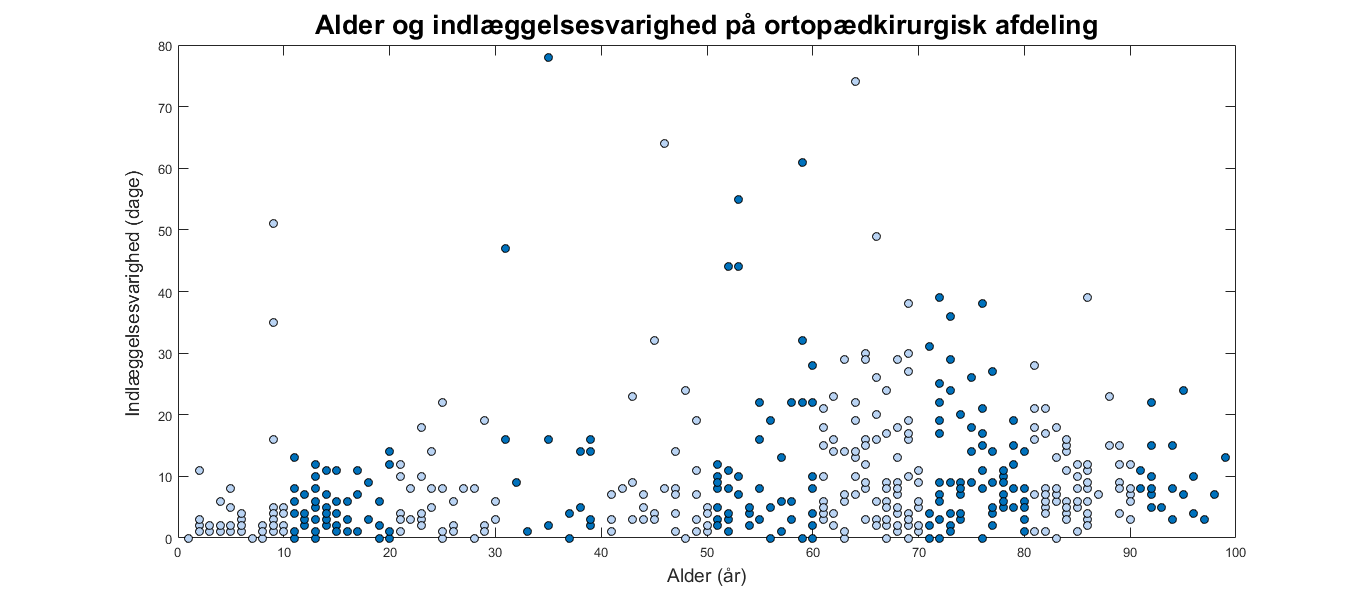
\includegraphics[scale=0.55]{figures/alderogindlaeg}
	\flushleft
	\caption{\textit{ *** TEKST TEKST TEKST *** }}
	\label{alderogindlaeggelse}
\end{figure}


\noindent
På \figref{alderogindlaeggelsese}  ***BLA BLA BLA**




Udover alder kan vægt ligeledes have en indflydelse på operationer foretaget på ortopædkirurgisk afdeling, da overvægt giver større risiko for blodpropper\cite{Ermonds2004}. Ved overvægt anbefales det derved at tabe sig før en eventuel operation. Foruden mindsket risiko ved opståen af komplikationer, kan smerter ligeledes reduceres ved vægttab.\cite{Nordjylland2014} På \figref{BMIogindlaeggelse} fremgår body mass index (BMI) samt indlæggelsesvarigheden i samme periode som \figref{alderogindlaeggelse}.


\begin{figure}[H]
	\flushleft 
	\centering
	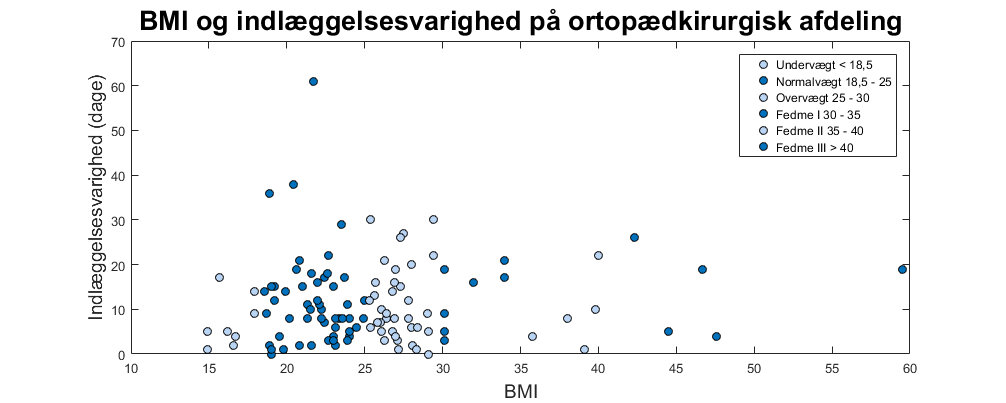
\includegraphics[scale=0.55]{figures/BMIogindlaeg}
	\flushleft
	\caption{\textit{ *** TEKST TEKST TEKST *** }}
	\label{BMIogindlaeggelse}
\end{figure}




\noindent
Af \figref{BMIogindlaeggelse} fremgår ***BLA BLA BLA** .\\




\noindent
Andre livsstilsfaktorer såsom rygning og alkohol kan have betydning for komplikationer under operationer. Rygning kan være medvirkende til at knogler og sår heler langsommere. Ved operationer, hvor der skal transplanteres knoglevæv, f.eks. rygoperationer, afhænger operationens resultat af, at knoglevævet heler rigtigt. Definitionen af en ikke ryger er en person, der har været røgfri i op til 6 måneder, det anbefales derfor at stoppe med at ryge 6 måneder før den planlagte operation.\cite{Nordjylland2014} Fordelingen af ryger, tidligere ryger samt ikke ryger og, hvilken betydning dette har for indlæggelsesvarigheden fremgår af \figref{rygningogindlaeggelse}.


\begin{figure}[H]
	\flushleft 
	\centering
	\includegraphics[scale=0.55]{figures/RYGNINGOGINDLÆGGELSESVARIGHED}
	\flushleft
	\caption{\textit{ *** TEKST TEKST TEKST *** }}
	\label{rygningogindlaeggelse}
\end{figure}


\noindent
Det ses af \figref{rygerogindlaeggelse} *** BLA BLA BLA ***


Som tidligere nævnt kan alkohol ligeledes medføre øget risiko for komplikationer under operationer. Herunder kan der opstå øget blødning under operationer samt infektioner i såret.\cite{Nordjylland2014} 


\begin{figure}[H]
	\flushleft 
	\centering
	\includegraphics[scale=0.55]{figures/alkohologindlaeggelse}
	\flushleft
	\caption{\textit{ *** TEKST TEKST TEKST *** }}
	\label{alkohologindlaeggelse}
\end{figure}


\noindent
Det ses af \figref{alkohologindlaeggelse} *** BLA BLA BLA ***


\subsubsection{Indgreb}
Som beskrevet i \ref{kap_OA} udføres flere operationstyper med forskellig varighed på ortopædkirurgisk afdeling, hvorfor det forventes at indlæggelsesvarigheden ligeledes er varierende. 


\begin{figure}[H]
	\flushleft 
	\centering
	\includegraphics[scale=0.55]{figures/opvsindlaegtid}
	\flushleft
	\caption{\textit{*** TEKST TEKST TEKST *** }}
	\label{opvsindlaegtid}
\end{figure}


\noindent
På \figref{opvsindlaegtid} fremgår *** BLA BLA BLA ***



\subsubsection{Tilgængelige kirurger}
Det kan i nogle tilfælde være nødvendigt at udsætte elektive patienters operationer, hvis et akut tilfælde opstår, hvorved kirurgen skal være til stede. Derved kan patienter indlæggelsesvarighed forlænges. Ved udsættelse af elektive patienter vil denne ofte få en ny tid hurtigst muligt. Den nye tid vil typisk være først på dagen, således risikoen for endnu en udsættelse mindskes.